\documentclass[bigger]{beamer}
\setbeameroption{show only notes}
\setbeamercolor{note page}{bg=white}
\setbeamercolor{note title}{bg=white}

\setbeamersize{text margin left=1cm, text margin right=1cm}
\setbeamertemplate{navigation symbols}{}
\setbeamertemplate{itemize items}{\textbullet}

\usepackage{graphicx}
\usepackage{helvet}
\renewcommand{\familydefault}{\sfdefault} % Sans-serif font like Arial
\setbeamerfont{frametitle}{size=\LARGE}
\setbeamerfont{framesubtitle}{size=\Large}
% \setbeamerfont{note page}{size=\footnotesize}

\setbeamertemplate{footline}{
  \leavevmode%
  \hfill
  
\includegraphics[height=0.5cm]{images/zengenti.png} % Adjust the height as needed
  \hspace{1em}
  \vspace{1em}
}

% \usebackgroundtemplate%
% {%
%   
\includegraphics[width=\paperwidth,height=\paperheight]{images/test_card.jpg}%
% }

\begin{document}
\title{All Code Sucks}
\subtitle{Why Bad Code is Everywhere and What to Do About It}
\author{Joe J Collins \\
  \href{mailto:j.collins@zengenti.com}{j.collins@zengenti.com} \\
  \href{https://linkedin.com/in/joejcollins}{linkedin.com/in/joejcollins}
}
\institute{
\includegraphics[height=1.5cm]{images/zengenti.png}}
\date{21 March 2024}

\begin{frame}[plain]
  \titlepage
  \note{Thanks for taking the time to join me tonight.\\
    I'm Big Joe from Zengenti.\\
    We are a small company in Shropshire. About 70 nerds.\\
    We do websites for universities and local authorities.\\
    I don't actually do any websites, I work in the hosting team.\\
    We maintain a private cloud to run websites.\\
    We use a combination of Ansible and Python\\
    maintaining about 3000 servers.\\
    But, tonight Matthew,\\
    I am going to talk about, \textbf{why all code sucks}.\\
    \vfil
    We all know good code,\\
    or at least we think we do.\\
    But I should probably define what I mean by sucky code.\\
  }
\end{frame}

\begin{frame}{What is sucky code?}
  \framesubtitle{}
  \begin{quote}
    ``Programs are meant to be read by humans and
    only incidentally for computers to execute.''\\
    \hfill --- Donald Knuth
  \end{quote}
  \bigskip
  \begin{quote}
    ``It is better to have clean code that doesn't work
    than crap code that does.''\\
    \hfill --- Robert C. Martin
  \end{quote}
  \note{My short answer is \dots \textbf{code that is hard to read}.\\
    No need take my word for it.\\
    Donald Knuth, the Yoda of Computer Science\\
    says that code is for humans to read\\
    and sometimes for computers to run.\\
    He is all about the readability.\\
    \vfil
    Uncle Bob Martin is more emphatic.\\
    He uses the term clean code.\\
    It is really a proxy for readability.\\
    He's says that readability is more important than working code.\\
    If you and understand it, then you can fix it,\\
    but if you can't understand it and it breaks, you can't fix it.
  }
\end{frame}

\begin{frame}{The Great Hunt for Non Sucky Code}
  
\includegraphics[width=\textwidth]{images/companies.png}
  \note{For about about 25 years now,\\
    I have been looking for code that doesn't suck.\\
    And trying to produce code that didn't suck.\\
    I have worked with scumbags and saints.\\
    And in companies both big and small.\\
    But pretty much all the code sucked.
    \vfil
    Maybe I just got unlucky.\\
    But I think I seeing a pattern.\\
    Maybe I should stop looking for the perfect code.\\
    And instead admit that all code sucks.\\
    And I should work out what to do about it.
    \vfil
    This does beg the question, why does it all suck?
  }
\end{frame}

\begin{frame}{Why Code Sucks}
  \framesubtitle{The Statistics Favour Suck}
  \begin{itemize}
    \item Half of everything is below average
      \pause
    \item Sturgeon's Revelation
      \pause
    \item The 2 Year Old Programmer Problem
  \end{itemize}
  \note<1>{
    On the whole I think the odds are against us.\\
    When we talk about code readability\\
    we are talking about a bell curve.\\
    Straight out of the gate,\\
    half of everything is going to be below average.\\
    Well, below the median.\\
    You don't have to be Francis Galton\\
    or any famous statistician\\
    to realize that.
  }
  \note<2>{Then there is Sturgeon's Law.\\
    Strugeon was explaining why most science fiction is low quality.\\
    And came up with the pithy response\\
    ``90\% of everything is shit''.\\
    The observation works here too.\\
    Only some things are really good.\\
    Put another way most of anything isn't good.
  }
  \note<3>{
    Then an issue perculiar to the programming business.\\
    The demand for programmers for the last 25 years\\
    has always outstripped supply.\\
    When I started out\\
    the average programmers experience was 3 years.\\
    And that hasn't changed.\\
    As more and more people have entered the business\\
    then have kept the average age down.\\
    There are a few old hands around but\\
    as a group we still don't have that much experience.
    \vfil
    So if the odds are against us\\
    maybe the organisations we work for will help.\\
    Well perhaps not.
  }
\end{frame}

\begin{frame}{Why Code Sucks}
  \framesubtitle{Organisations Tend To Suck}
  \begin{itemize}
    \item Software Startups
      \pause
    \item Summer Student Projects
      \pause
    \item Prototypes in Production
      \pause
    \item The New Project Effect
      \pause
    \item The Agile Manifesto
  \end{itemize}
  \note<1>{
    The romantic image of a software startup is\\
    a couple of guys in a garage.\\
    I have actually see this quite a bit.\\
    For most start ups the two guys are the dad and the son.\\
    The dad is the salesman.\\
    And the son is the programmer,\\
    who's typically been excluded from school for some reason.\\
    Writing readable code is not on their agenda.\\
    In fact reading plain English is not on their agenda.\\
    The third employee?\\
    The son's best mate from school who was also excluded.
  }
  \note<2>{
    The other kind of startup I have seen occurs in big companies.\\
    The summer student project.\\
    Alternatively called the unsupervised use of new technology.\\
    All the experienced programmers are on holiday or busy.\\
    So they give the new technology to the summer students,\\
    who give it a go.\\
    If it runs they put it into production.
  }
  \note<3>{
    This last point is also a general point.\\
    Any software that appears to work goes into production.\\
    Not because anyone thinks it's a good idea\\
    but because there is a commercial imperative.\\
    Having learnt from the prototype,\\
    the plan was to throw it away and build it for real.\\
    But that never happens.\\
    It is always put into production.\\
    And lives forever.
  }
  \note<4>{
    So, say you start a new project,\\
    well resourced with all the best intentions.\\
    The organisation is still against you.\\
    Who is available to work on the project?\\
    Anyone who is new or is on the bench.\\
    This isn't necessarily a bad thing.\\
    The average age of the team that\\
    helped put Neil Armstrong to the moon was 28.\\
    But they were all new to the business.\\
    The experienced engineers all had jobs\\
    and why take a risk on a new project?
  }
  \note<5>{
    Then there is Agile Management Practice \ldots\\
    it was such a great idea.\\
    We should respond to change over following the plan.\\
    It didn't say we shouldn't plan.\\
    But I was there 25 years ago,\\
    I was there the day the strength of Men failed\\
    and we deliberate misread the Agile Manifesto\\
    as `no need plan'.\\
    Just start programming!
    \vfil
    And as if this wasn't bad enough,\\
    I would say that suck is actually built into human psychology.
  }
\end{frame}

\begin{frame}{Why Code Sucks}
  \framesubtitle{The Psychology of Suck}
  \begin{itemize}
    \item The Illusion of Explanatory Depth
      \pause
    \item The Lake Wobegon Effect
      \pause
    \item Availability Bias
  \end{itemize}
  \note<1>{
    I think I am an intelligent person.\\
    I think I can understand most things.\\
    But my understanding is only a deep as it is.\\
    I am completely unaware of my ignorance.\\
    Because I am ignorant of it.\\
    I believe I understand things more than I do.\\
    It is unavoidable.\\
    But writing code is about explaining things in detail.\\
    And it does nothing but expose how little I know.
  }
  \note<2>{
    Add to this the Lake Wobegon Effect.\\
    Named after the fictional town,\\
    where all the women are strong, all the men are good-looking,\\
    and all the children are above average.\\
    93\% of drivers rate themselves in the top 50\% of driving ability.\\
    I think the code I write is above average.\\
    but is probably isn't.
    \vfil
    My judgement is clouded by my own ego.
    }
  \note<3>{
    A couple of years ago we used a code analysis tool on our code.\\
    To my surprise is said most of the code as good.\\
    But it pointed to the five worst files.\\
    Those were the files I spent most of my time working on.\\
    If by some miracle your code is great,\\
    you will only ever work on the bad code.\\
    Those will be the bits you remember.\\
    For practical purposes you will only ever see the bad code.\\
    So you think all code sucks.
    \vfil
    So what to do about it?
  }
\end{frame}

\begin{frame}{What Not To Do}
  \framesubtitle{}
  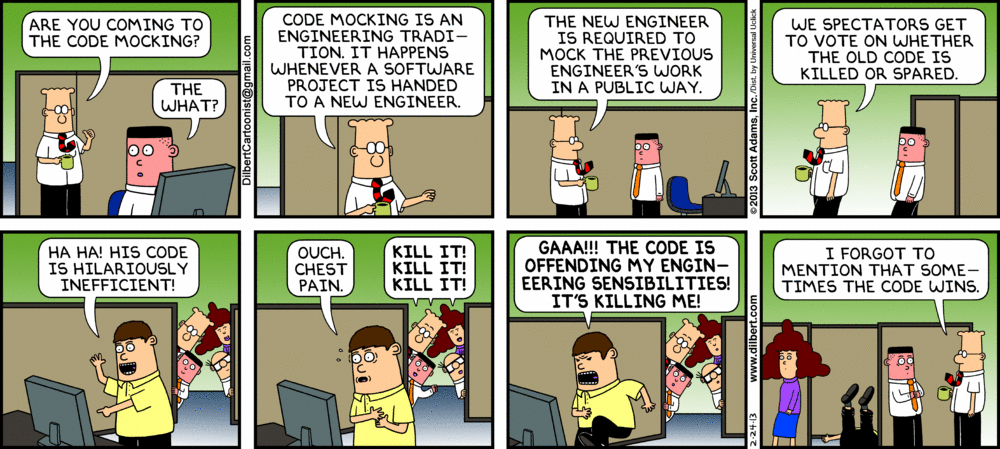
\includegraphics[width=\textwidth]{images/code-mocking.png}
  \note{What not to do is the ritual code mocking.\\
    Everyone is doing their very best\\
    with the time, resources and knowledge they have.\\
    If we assume the code will suck and we just have to work with it.\\
  Then we can start to work out what to do about it.}
\end{frame}

\begin{frame}{What To Do}
  \framesubtitle{Based on the work of Michael Feathers}
  \begin{itemize}
    \item Put the code in a vice (a test harness)
    \item Get ahead of the offending code with a feature flag
    \item Side by side rewrite
  \end{itemize}
  \note{
  }
\end{frame}

\begin{frame}{The Challenge}
  \framesubtitle{Where I need your help}
  \begin{quote}
    ``It's not that hard...''\\
    \hfill --- Billy Beane
  \end{quote}
  \bigskip
  \begin{quote}
    ``It's incredibly hard''\\
    \hfill --- Ron Washington
  \end{quote}
  \bigskip
  \note{To quote Moneyball,\\
    the challenge is both easy and difficult.\\
    Taken
  }
\end{frame}

\begin{frame}[plain]
  \centering
  {\Huge \bfseries Thank You!}\\[1cm]
  {\large Joe J Collins} \\[0.5cm]
  
\includegraphics[height=1.5cm]{images/zengenti.png}
\end{frame}

\end{document}
